\subsection{Présentation du problème}
	Comme nous l'avons vu dans le chapitre précédent, les sphères isothermes ne sont pas une solution satisfaisante, du fait de leurs masses infinies.
	Nous allons présenter dans ce chapitre une solution de sphère isotherme intégrée sur un support borné. Cette solution est toujours obtenue en recherchant des maxima  de l'entropie statistique de Boltzmann:
	\begin{align*}
		S(f) = - k_B \int f \ln f \vdp\vdr
	\end{align*}
	mais pour une fonction $f$ possédant un support borné. Ce dernier est par exemple une boule (souvent appelée boîte, d'où le nom du chapitre) définie comme :
	\begin{align}
		B = \left\{ \vec{r} \in \mathbb{R}^3\ ;\ \left|\vec{r}\right| < R\right\}
	\end{align}
	où $R$ est le rayon de la boule support de $f$. Dans la suite, nous noterons $\mathbb{I}_{B_R}$ la fonction indicatrice sur cette boule.

\subsection{Obtention des équations}
	La fonction de distribution d'une sphère isotherme en boîte, s'écrit (voir par exemple \cite{CoursJP}) :
	\begin{align}
		f^+(E) = \left(\frac{2\pi\alpha^2m}{\beta}\right)^{-3/2}e^{-\beta E}\times\mathbb{I}_{B_R}
	\end{align}
	où $\alpha$, en mètre, et $\beta=(k_B T)^{-1}$, en Joule, sont des multiplicateurs de Lagrange imposés
	par les contraintes respectives de masse $M$ et d'énergie totale $H$ finie que nous imposons toujours au système.
	Ils assurent également la normalisation de la fonction de distribution.
	% La quantité \mbox{$E = \frac{p^2}{2m} - m\psi(r)$} est l'énergie d'une particule test de masse $m$ se déplacant dans
	% le potentiel $\psi$ créé par la sphère isotherme.
	Le calcul de la densité de masse donne alors \mbox{$\rho(r) = \frac{m}{\alpha^3}e^{-\beta m \psi(r)}\times\mathbb{I}_{B_R}$}. % \psi'(r)}$}, dans la suite nous utiliserons :
	%\mbox{$\psi'(r) = \psi(r) - \psi(0)$}~\footnote{pour faciliter les calculs dans les variables Milne définies ci-dessous}.
	L'équation de Poisson s'écrit :
	\begin{align}
		 \frac{1}{x^2}\frac{d}{dx}\left(x^2\frac{d h}{dx}\right) = e^{-h} \times\mathbb{I}_{B_R} \notag
	\end{align}
	où nous avons utilisé l'adimensionnement  :
	\begin{align}
		x &= \frac{r}{r_0}\mathrm{ avec }\ r_0 = \sqrt{\frac{\alpha^3}{4\pi G m^2\beta}}e^{-\frac{m\beta\psi(0)}{2}} \label{toto11} \\
		h &= m\beta\psi(x) - m\beta\psi(0) \label{toto12}
		\end{align}
		Il est important de noter que l'inconnue du problème $h(x)$ est différente de $y(x)$ utilisée pour la présentation du problème de la sphère isotherme illimitée. Nous avons ici $h(0) = 0$ alors que $y(0) = m\beta\psi(0)$.
		
		En notant par un $^\prime$ toutes les dérivées par rapport à la variable $x$, nous introduisons les variables dites de \textsc{Milne :}
		\begin{align}
			\begin{cases}
			v = x \dfrac{d h}{dx} = x \x{h} \\
			\\
			u = \dfrac{e^{-h} x}{h'} = \dfrac{e^{-h} x^2}{v}
		\end{cases}\label{syst_uv}
		\end{align}
		
Un calcul simple donne alors :
\begin{align}
	\dfrac{d(xv)}{dx} = uv \;\;\Rightarrow\;\; \x{v} = \frac{v \left( u - 1\right)}{x} \notag
\end{align}
La dérivée de $u$ s'obtient directement à partir de sa définition, nous trouvons:
	$$\begin{cases}
		\x{v} = \dfrac{v \left( u - 1\right)}{x} \\
		\x{u} = \dfrac{u}{x}\left(3 - v - u\right)
	\end{cases} \label{systdudv}$$
	
	que nous pouvons écrire de façon compacte:
	\begin{align}
		\dfrac{d v}{d u} = \dfrac{v \left( u - 1\right)}{u \left(3 - u - v\right)}
		\label{eqdudv}
	\end{align}
	La courbe résultant de cette équation, tracée dans le plan $\left(u, v\right)$, forme le diagramme
	de Milne. L'étude de ce diagramme permet d'accéder à de nombreuses caractéristiques de la sphère isotherme en
	boîte. L'équation~\refeq{eqdudv} ne peut être résolue explicitement mais sa solution peut être obtenue
	numériquement: il faut pour cela préciser les conditions au bord et au centre du système; ce qui est l'objet de la
	section suivante.
	

\subsection{Conditions au centre et sur le bords de la sphère}
	Pour obtenir les conditions initiales permettant la résolution de l'équation~\ref{eqdudv}, nous devons obtenir les conditions aux limites pour la sphère isotherme en boîte.
\subsubsection{En $x = 0$}
	Pour ce faire, nous nous plaçons dans le voisinage de $x=0$, et faisons donc des développements limités de la variable $h$ représentant le potentiel.
	Cela nous permettra d'obtenir le comportement approché de $u(x)$ et de $v(x)$ au centre.
	Nous avons donc :
	\begin{eqnarray*}
		h(x) = h(0) + \x{h}(0)x + \frac{d^2 h}{dx^2}(0)\frac{x^2}{2!} + \frac{d^3 h}{dx^3}(0)\frac{x^3}{3!} + o(x^3) = ax^2 + bx^3 + o(x^3)
	\end{eqnarray*}
	En effet, \mbox{$h(0) = m\beta\left(\psi(0) - \psi(0)\right) = 0$} et \mbox{$\x{h}(0) = m\beta\x{\psi}(0) = 0$} car \mbox{$\x{\psi} = r_0\frac{d \psi}{dr}\propto F$},
	$F$ étant la force s'appliquant sur la particule test.
	Au centre de la sphère, les forces qui s'appliquent à une particule test s'opposent les unes aux autres, d'où $\x{h}(0) = 0$.

	Les variables $u$ et $v$ vont alors se développer comme :
	\begin{eqnarray}
		v &=& x\x{h} = 2ax^2 + 3bx^3 + o(x^3)\label{vDL} \\
		u &=& \frac{x^2e^{-ax^2 - bx^3 + o(x^3)}}{2ax^2 + 3bx^3 + o(x^3)} \\
		  &=& \frac{1 - ax^2 - bx^3 + o(x^3)}{2a + 3bx +o(x)} \\
		  &=& \frac{1}{2a} - \frac{3b}{4a^2}x + o(x)\label{uDL}
	\end{eqnarray}
	Nous utilisons ensuite l'équation de Poisson pour déterminer, par identification, les valeurs de $a$ et de $b$ :
	\begin{eqnarray}
		\x{\left(xv\right)} = 6ax^2 + 12bx^3 + o(x^3) = uv = x^2 + o(x^3)\label{PoisDL}
	\end{eqnarray}
	D'où :
	\begin{eqnarray}
		\left\{\begin{array}{l}
			a = \frac{1}{6} \\
			b = 0
		\end{array}\right.
	\end{eqnarray}
	Maintenant que nous avons nos développements, nous en déduisons les conditions initiales :
	$$(u,v) \substack{\longrightarrow \\ r\to 0} (3,0)$$

\subsubsection{Sur le bords de la sphère : $r = R$}
	Soit $X = \frac{R}{r_0}$. Nous allons tenter d'exprimer nos variables $u$ et $v$ au point $X$ en fonction des quantités connues du problème,
	telles que l'énergie totale $H$, la masse totale $M$, le rayon de la sphère $R$.
	Et, selon la description canonique ou micro canonique choisie, en fonction de la température cinétique du système.

	On introduit les constantes adimensionnées suivantes :
	\begin{eqnarray*}
		\left\{\begin{array}{l}
			\lambda = - \frac{H R}{G M^2} \\
			\\
			\mu     = \frac{m\beta GM}{R}
		\end{array}\right.
	\end{eqnarray*}
	où $\lambda$ représente l'énergie adimensionnée et $\mu$ l'inverse de la température adimensionnée.

	Au bord du système, nous pouvons écrire que $\frac{d \psi}{dr} \equiv \frac{GM}{R^2}$~\footnote{Théorème de Gauss}. De plus :
	\begin{eqnarray*}
		\x{h}(X) = m\beta r_0 \frac{d \psi}{dr} = m\beta r_0 \frac{GM}{R^2} = \frac{\mu}{X} \Rightarrow \mu = X\x{h}(X)
	\end{eqnarray*}
	Or $v(X) = X\x{h}(X)$, d'où :
	\begin{eqnarray}
		v\left(X\right) := v_m = \mu\label{vmmu}
	\end{eqnarray}

	Il nous reste l'énergie à exprimer.
	Pour cela, nous allons commencer par calculer l'énergie totale $H$ à l'aide du théorème du Viriel adapté à une sphère isotherme en boîte~\footnote{Pour un système tronqué, le calcul permettant d'arriver au théorème du Viriel fait apparaître des termes dû aux intégrations par partie qui vont rester.} :
	\begin{eqnarray}
		2T + W = \frac{4}{3}\pi R^3 P_e
	\end{eqnarray}
	avec $P_e$ la pression qui s'exerce sur le bord de la sphère.
	L'énergie cinétique s'écrit \mbox{$K = \frac{1}{2}mv^2 = \frac{3}{2} N k_B T = \frac{3}{2} \frac{M}{m} k_B T$}.
	Donc :
	\begin{eqnarray*}
		H &=& K + W = \frac{3}{2} \frac{M}{m\beta} + \frac{4}{3}\pi R^3 P_e - 2K \\
		  &=& -\frac{3}{2} \frac{M}{m\beta} + \frac{4}{3}\pi R^3 P_e \\
		\Rightarrow \lambda &=& \frac{3}{2}\frac{MR}{m\beta GM^2} - \frac{4}{3}\pi R^3 P_e \frac{R}{GM^2}
	\end{eqnarray*}
	Une sphère isotherme est un système barotropique. Elle a donc une équation d'état polytropique d'indice 1 : $P = \frac{\rho(r)}{m\beta} \Rightarrow P_e = \frac{\rho(R)}{m\beta}$ que nous remplaçons :
	\begin{eqnarray}
		\lambda &=& \frac{3}{2}\frac{1}{X\x{h}(R)} - \frac{4}{3}\pi R^3 \frac{\rho(R)}{m\beta} \frac{R}{GM^2} \notag \\
			&=& \frac{3}{2}\frac{1}{X\x{h}(R)} - \frac{4}{3}\pi R^3 \frac{e^{-h(R) + m\beta\psi(0)}}{\alpha^3\beta} \frac{R}{GM^2} \notag \\
			&=& \frac{3}{2}\frac{1}{X\x{h}(R)} - \frac{4}{3}\pi R^3 \frac{4\pi G \beta m^2 e^{\beta m \psi(0)}}{\alpha^3} r_0^2\frac{e^{-h(R)}}{(\x{h}(R))^2} \notag \\
			&=& \frac{3}{2}\frac{1}{X\x{h}(R)} - \frac{e^{-h(R)}}{(\x{h}(R))^2}\label{lamum}
	\end{eqnarray}

	Nous avons ensuite, par substitution, les valeurs maximales $u_m$ et $v_m$ de $u$ et $v$ en fonction des paramètres du problème :
	\begin{eqnarray}
		\label{uv_max}
		\fbox{$
		\left\{\begin{array}{l}
			v_m = \mu \\
			u_m = \frac{3}{2} - \lambda \mu
		\end{array}\right.
		$}
	\end{eqnarray}



\subsection{Droites de Padmanabhan et diagramme de Milne}
	% On peut facilement éliminer $\mu$ dans le système~\ref{uv_max} et obtenir
	Les $\mu$ dans le système~\refeq{uv_max} peuvent facilement s'éliminer et nous obtenons:
	\begin{align}
		v_m = \frac{3}{2\lambda} - \frac{u_m}{\lambda}\label{droitePb}
	\end{align}
	Cette relation montre que si l'on ne fixe que la valeur de $\lambda$,  les couples $(u_m,v_m)$  se répartissent
	dans le plan $(u,v)$ le long d'une droite de pente $-1/\lambda$, dite de Padmanabhan en référence à sa remarque
	dans l'article \cite{1989ApJS...71..651P}. Nous remarquons aussi que toutes ces droites passent par le point
	$(\frac{3}{2},0)$.
	
	Le choix de $\lambda$ est indépendant de la valeur de la température, le point $(u_m,v_m)$ associé à la sphère
	isotherme en boite de rayon $R$, de masse $M$, d'énergie $H$ et de température $\beta$ se trouve donc à
	l'intersection de la droite de Padmanabhan fixée par $\lambda$ et de la courbe $v(u)$ solution de
	l'équation~\refeq{eqdudv}. 
	
	
	Cette courbe est obtenue numériquement à l'aide d'un solveur Runge-Kutta d'ordre 4, en utilisant les variables adimensionnées, le
	seul paramètre physique pour la résolution étant la valeur de $X$ caractérisant le rayon et la température de la
	sphère.  L'ensemble de ces courbes et des droites de Padmanabhan correspondantes sont représentées sur la figure~\ref{Milne}.
	Nous constatons que plus la valeur de $R$ augmente, plus la courbe
	solution est longue et finit par s'enrouler dans une spirale convergeant vers un point. Ce point correspond au
	cas $R\to\infty$ et donc celui de la \textsc{sis}.
	% Pour une température fixée, nous constatons que plus la valeur de $R$ augmente plus la courbe
	% solution est longue et finit par s'enrouler dans une spirale convergeant vers un point. Ce point correspond au
	% cas $R\to\infty$ et donc celui de la \textsc{sis}.
	
	À l'inspection de ce diagramme et de ces droites, nous comprenons aisément que l'on ne peut pas mettre
	n'importe quelle sphère isotherme dans n'importe quelle boîte. %qu'elle boîte.

	En effet, si l'on impose des valeurs de $R$,
	$M$ et $H$ qui donnent une valeur trop grande $\lambda>\lambda_c$, la droite ne pourra pas avoir d'intersection
	avec la courbe. Cette intersection qui aurait fixé le dernier paramètre, la température, n'existant pas il en va
	de même de la sphère isotherme en boîte possédant ces caractéristiques physiques.
	
	Nous remarquons même l'existence d'une seconde valeur caractéristique $\lambda_0$ telle que :
	\begin{itemize}
		\item si $\lambda < \lambda_0$ : il n'existe qu'une seule et unique sphère isotherme possible;
		\item si $\lambda \in \left[\lambda_0,\lambda_c\right]$ : il existe plusieurs possibilités;
		\item si $\lambda > \lambda_c$ : il n'y a plus d'intersection possible !
	\end{itemize}

Comme nous allons le voir dans la prochaine section, cette multiplicité de possibilités est associée à la stabilité des sphères concernées.

	\begin{figure}[h!]
		\begin{minipage}[b]{0.40\linewidth}
			\centering 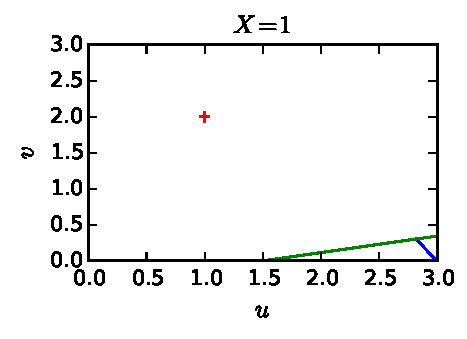
\includegraphics{graphe/milne_X1.pdf}
		\end{minipage}\hfill
		\begin{minipage}[b]{0.48\linewidth}
			% \centering \includegraphics[scale=0.60]{graphe/r_max-5.pdf}
			\centering 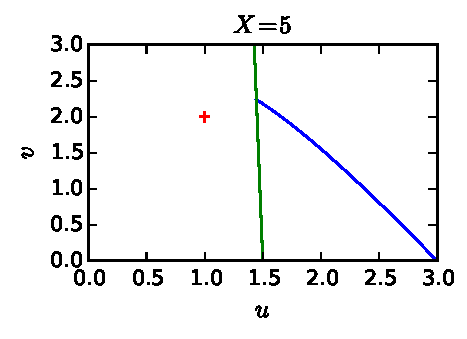
\includegraphics{graphe/milne_X5.pdf}
		\end{minipage}
		\begin{minipage}[b]{0.40\linewidth}
			% \centering \includegraphics[scale=0.60]{graphe/r_max-10.pdf}
			\centering 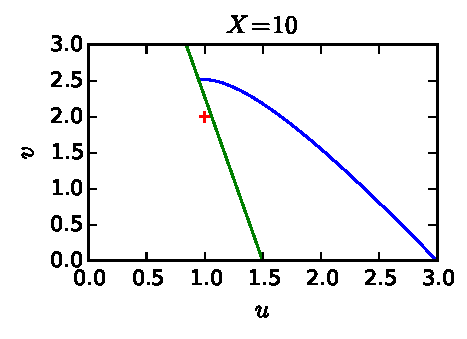
\includegraphics{graphe/milne_X10.pdf}
		\end{minipage}\hfill
		\begin{minipage}[b]{0.48\linewidth}
			% \centering \includegraphics[scale=0.60]{graphe/r_max-300.pdf}
			\centering 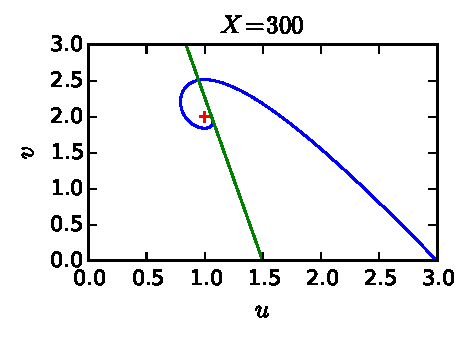
\includegraphics{graphe/milne_X300.pdf}
		\end{minipage}
		\caption{Diagramme de Milne pour $X=1$, $X=5$, $X=10$ et pour $X=300$. La sphère isotherme est
		représenté par la courbe bleue, la courbe de Padmanabhan est en vert et la \textsc{sis} en rouge.}
		\label{Milne}
	\end{figure}
